%
% LaTeX template for prepartion of submissions to PLDI'16
%
% Requires temporary version of sigplanconf style file provided on
% PLDI'16 web site.
% 
\documentclass[pldi]{sigplanconf-pldi16}
% \documentclass[pldi-cameraready]{sigplanconf-pldi16}

%
% the following standard packages may be helpful, but are not required
%
\usepackage{SIunits}            % typset units correctly
\usepackage{courier}            % standard fixed width font
\usepackage[scaled]{helvet} % see www.ctan.org/get/macros/latex/required/psnfss/psnfss2e.pdf
\usepackage{url}                  % format URLs
\usepackage{listings}          % format code
\usepackage{enumitem}      % adjust spacing in enums
\usepackage[colorlinks=true,allcolors=blue,breaklinks,draft=false]{hyperref}   % hyperlinks, including DOIs and URLs in bibliography
% known bug: http://tex.stackexchange.com/questions/1522/pdfendlink-ended-up-in-different-nesting-level-than-pdfstartlink
\newcommand{\doi}[1]{doi:~\href{http://dx.doi.org/#1}{\Hurl{#1}}}   % print a hyperlinked DOI

\usepackage{array,multirow,graphicx}
\usepackage[usenames,dvipsnames]{color}
\usepackage[latin1]{inputenc}
\usepackage{tikz}
\usetikzlibrary{shapes,arrows}
\newcommand{\ruzica}[1]{\textcolor{Magenta}{\textsf{RP}: #1}}
\newcommand{\markk}[1]{\textcolor{Blue}{\textsf{MS}: #1}}
\newcommand{\alex}[1]{\textcolor{Orange}{\textsf{AR}: #1}}


\def\ourTool/{our tool}
\def\lhask/{LiquidHaskell}

\newcommand{\codeinline}[1]{\lstinline[basicstyle=\small]{#1}}



\usepackage{comment}

\usepackage{graphicx}

\definecolor{identifierColor}{rgb}{0.65,0.16,0.16}
\definecolor{comment_color}{rgb}{0.40,0.46,0.3}
\definecolor{num_color}{gray}{0.55}

\lstset{
  basicstyle=\footnotesize,
  breaklines=true,
  frame=bottomline,
  language=haskell,
  %identifierstyle=\color{identifierColor},
  morecomment=[l][\color{comment_color}\ttfamily]{--},
  backgroundcolor=\color{white},   % choose the background color; you must add \usepackage{color} or \usepackage{xcolor}
  breakatwhitespace=false,         % sets if automatic breaks should only happen at whitespace
  %captionpos=b,                    % sets the caption-position to bottom
  %commentstyle=\color{mygreen},    % comment style
  %frame=single,	                   % adds a frame around the code
  keepspaces=true,                 % keeps spaces in text, useful for keeping indentation of code (possibly needs columns=flexible)
  keywordstyle=\color{blue},       % keyword style
  otherkeywords={*,let, Server, Replication, FaultGraph, rankRCG, print, fialProb, goal, ...},           % if you want to add more keywords to the set
  numbers=left,                    % where to put the line-numbers; possible values are (none, left, right)
  numbersep=5pt,                   % how far the line-numbers are from the code
  numberstyle=\tiny\color{num_color}, % the style that is used for the line-numbers
  rulecolor=\color{black},         % if not set, the frame-color may be changed on line-breaks within not-black text (e.g. comments (green here))
  showtabs=false,                  % show tabs within strings adding particular underscores
  stepnumber=1,                    % the step between two line-numbers. If it's 1, each line will be numbered
  stringstyle=\color{mymauve},     % string literal style
  %title=\lstname                  % show the filename of files included with \lstinputlisting; also try caption instead of title
  mathescape=true,
  tabsize=3,
  literate=*{->}{{\textcolor{blue}{$\to$}}}{1}
           {<-}{{\textcolor{blue}{$\leftarrow$}}}{1}
}
  
  
%\usepackage{minted}
%\usepackage{tcolorbox}
%\usepackage{etoolbox}
%\BeforeBeginEnvironment{minted}{\begin{tcolorbox}}%
%\AfterEndEnvironment{minted}{\end{tcolorbox}}%

\begin{document}

\title{Natural Program Synthesis from Examples in Haskell}

%
% any author declaration will be ignored  when using 'pldi' option (for double blind review)
%

\authorinfo{Person 1 \and Person 2}
{\makebox{Department of Computer Science} \\
\makebox{Yale University}  \\
\makebox{A Place, AS 12345}}
{\{person1,person2\}@cs.auniv.edu}


\maketitle

\begin{abstract}
We present a new programming-by-example technique that efficiently synthesizes natural, readable fitting functions that combine user-defined higher-order functions with standard and third-party library code.

The search works by \textit{dismantling} higher-order functions in order to deduce suitable refinement types. These refinement types are then used to prune the search space of possible higher-order functions for a given example set. Since refinement type under-approximate, we can apply Liquid Haskell to arbitrary syntax extensions while still preserving soundness.

We evaluate an implementation of our tool against a large set of synthesis examples including lists, trees, maps, and specialized musical score data structures. This evaluation demonstrates the scalability and versatility of this approach.
\end{abstract}

\section{Introduction} 
\label{intro}

A core part of the functional programming experience is writing higher order functions. The functional programming approach encourages specifying general behaviors in the form of abstract, higher-order functions first, and filling in details with first-order functions later. Many users write higher order functions first, then combine them in interesting and useful ways. Library authors often provide users with many higher order functions to allow users more easily write their applications. With this in mind, we provide a synthesis engine that is able to leverage user defined higher order functions.

Since users write higher order functions with a deep understanding of the domain, using them will produce code that is more idiomatic and easier to understand then using generic higher order functions. Additionally, fewer examples are needed because we have access to the domain specific knowledge encoded by the user library.


A core part of the functional programming experience is writing higher order functions. The functional programming approach encourages specifying general behaviors in the form of abstract, higher-order functions first, and filling in details with first-order functions later.

A core part of the functional programming experience is writing higher order functions. Many users write higher order functions first, then combine them in interesting and useful ways. Library authors often provide users with many higher order functions to allow users more easily write their applications. With this in mind, we provide a synthesis engine that is able to leverage user defined higher order functions.

Since users write higher order functions with a deep understanding of the domain, using them will produce code that is more idiomatic and easier to understand then using generic higher order functions. Additionally, fewer examples are needed because we have access to the domain specific knowledge encoded by the user library. The user can also use this tool to synthesize new, simpler versions of a program. 

\begin{lstlisting}
-- User has their own library of fxns
f :: a -> [a]
f x = [x,x]

-- and wants to synthesize stutter
exs :: [[Int] :-> [Int]]
exs = [[1, 2, 3] :-> [1, 1, 2, 2, 3, 3]]

-- or find a more natural stutter program
exs :: [[Int] :-> [Int]]
exs = [[1, 2, 3] :->
       foldl (\xs x -> xs++[x,x]) [1,2,3]]
      
-- the system will find
prog  = concatMap f
prog' = concatMap (replicate 2) 
\end{lstlisting}



If a user is importing a library, they can also synthesize programs that use those function. As an example, we show code to transpose a music value from the Euterpea DSL for music in haskell. The solution uses the builtin functions \texttt{mMap} (mapping over music values) and \texttt{trans :: Int->Music Pitch->Music Pitch} to transpose a Music Pitch by a value.

\begin{lstlisting}
import Euterpea

exs :: [Music Pitch :-> Music Pitch]
exs = [ (c 4 qn  :+: d 4 qn) :->
        (ef 4 qn :+: f 4 qn) ]
        
prog = mMap (trans 3)
\end{lstlisting}


\section{Problem Formulation} 
\label{problem}


Synthesizing correct programs is a well researched problem; however, if programming-by-example is to become a mainstream tool for programmers, the synthesized code must be easy for a human to read and modify. 
The aim of \ourTool/ is to synthesize programs from examples that utilize user defined code in a clear and concise.
We focus particularly on data structure manipulation problems that can be solved with higher order functions.

\subsection{Example Syntax}
Formally speaking, an \textit{example} is a pair of values with distinguished ``input'' and ``output'' elements, and an \textit{example set} is a set of examples all of whose inputs are of like type, and all of whose outputs are of like type. The output type does not necessarily match the input type.

A user supplies examples via a custom pair constructor \texttt{:->}. This operator is used to differentiate between generic pairs and examples, but does not confer any additional structure. We require all higher order functions to be of a unified signature \texttt{$\_ \to * \to *$}, where the final kind of the signature is a function mapping the input type to the output type. Here, a kind is understood to be the type of a type constructor, in this case \texttt{$\to$}, which constructs a function type from two other types.

The practical consequence of this format is that a user must partially uncurry (collapsing trailing function arguments into a single tuple argument) any higher-order function they are interested in using during synthesis.
This also means that any type variable appearing in the higher-order function must be accounted for in the input and output types so that all type variables in its signature can be resolved.
This allows us to conclude that any types that are between the input and first order function will be static initial values, which can be assigned using the process described in Section \ref{makeFxns}.
This is a simple procedure that makes use of the user's domain knowledge of which parameters to the function will be given by the examples; consider:

\begin{lstlisting}
zipWith' :: (a -> b -> c) -> ([a], [b]) -> [c]
zipWith' f (xs,ys) = zipWith f xs ys
\end{lstlisting}

\subsection{Solution Space}\label{solnSpace}
By formally defining the space of functions we are interested in synthesizing, we can this definition to prove some properties on the algorithm.
In particular we show in Section \ref{sound} that \ourTool/ is complete for this subset of functions.

the solutions \ourTool/ supports synthesizing are higher-order data structure manipulation programs.
The higher-order functions take a component function that is a first-order function, for example \codeinline{(+)}.
The solution programs can be expressed as:
% up to reordering of terms (we dont actually support this, should we really include this)

\begin{lstlisting}
solution ::
           (* -> types)  -- Component Function
        ->  types        -- Initial Values
        ->  *            -- Input
        ->  *            -- Output
types = * | * -> types
-- * matches on type variables and constructors.
\end{lstlisting}

Generally, the component function is applied across the \textsf{input} data structure, which the \textsf{solution} uses to construct an \textsf{output} data structure or reduction. As we will argue in Section \ref{evaluation} this set is expressive enough to support the classic \texttt{map}, \texttt{filter}, and \texttt{fold} functions, as well as higher order functions found in imported modules and user-supplied code.

Our goal is to create a synthesis procedure that is easily portable across full implementations of functional languages (Haskell, OCaml, etc), so we prefer using a type directed approach to synthesis over explicit code analysis whenever possible. This increases the portability and longevity of our system. For this implementation we target Haskell, detailing the exact modifications needed to expand this to other languages in Section \ref{languageSupport}.  

%Our algorithm does not explicitly try to fit component functions to the examples. Instead, we leverage a promising body of existing work in synthesizing top-level, first-order functions \cite{potential, reviewers}. While it is out of scope to go in to detail, we will briefly discuss the integration of these synthesis procedures in Section \ref{conclusions}.

%The liquidHaskell predicate applied to this signature will be of the effect of \texttt{len([a],[b]) = len([c])}.


\begin{figure}[t]
  \centering
  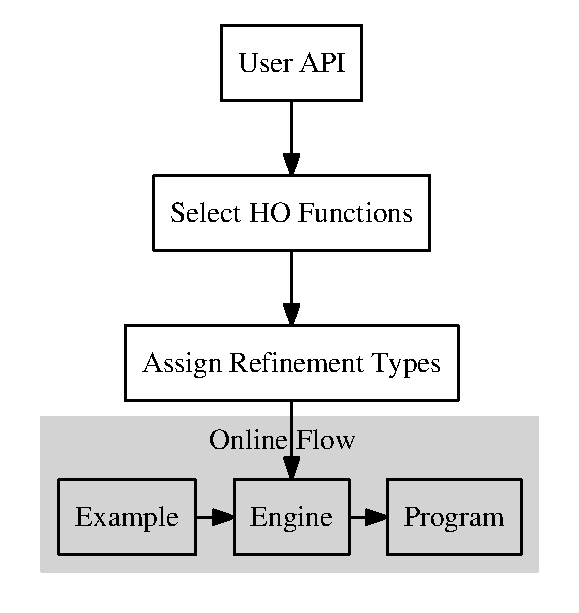
\includegraphics[width=0.45\textwidth]{algo}
  \caption{High-level structure of the algorithm.}
  \label{fig:high_level_overview}
\end{figure}

In this section, we give a high-level description of each component of our algorithm. Figure~\ref{fig:high_level_overview} below illustrates the ways in which these components interact. Broadly speaking, there are two main stages in the algorithm. The offline phase gathers the higher order declarations visible in the APIs and user-provided code, and assigns refinement types to them to build a custom synthesis \textit{engine}. This engine is then used during the online phase of the algorithm to search for functions that fit a set of supplied examples.

During the offline phase, the algorithm first scans the user-provided code, the libraries it imports, and the standard library to gather all of the functions and global values visible to the program. Then, it selects the higher-order functions from the set of all functions and values, and uses Liquid Haskell \cite{liquidhaskell} to assign refinement types to each one. Finally, each higher-order function is assigned a weight based on locality. User-defined functions are given the highest priority, while direct imports are given less, and the standard libraries are given the least. Together with the first-order functions and values, these triples of higher-order functions with their refinement types and weights are collected to produce a synthesis engine.

Once this stage is complete, the user can make online queries to the synthesis engine, which will search the space of constructable functions for those that fit the input examples. First, the engine computes a refinement type that fits the examples. This type is matched against the refinement types of the known higher-order functions, and the weights of each known function are adjusted based on how close the types match, if at all.

Once the candidate higher order functions have been chosen, the synthesis engine performs a best-first search for a program that fits all of the input and output examples by composing the candidates with first-order functions. For example, the higher-order function \texttt{map} might be supplied the \texttt{length} function if the example inputs are lists of lists of integers and the output examples are all lists of integers. The programs that are examined during the search are evaluated against the example set and are reported to the user as they match. Because the weights favor local declarations, the highest-ranked programs are likely to be the most idiomatic.

\subsection{Refinement type inference}

%>  filter ishigherOrder tys
We first collect all of the type signatures from our sources (user code, imports, and standard library). We filter through these to select only the higher order functions. Because in Haskell the function type constructor (->) is right binding, any higher order functions must have parenthesis in the type signature, which provides a convenient filtering predicate.

%> let uHOTyps = f 3000 typSigs
%> let iHOTyps = f 2000 importSigs
%> let pHOTyps = f 1000 preludeTypSigs
In order to rank the higher-order functions we assign weights based on their source location. User-defined functions are given the highest priority, while direct imports are given less, and the standard libraries are given the least. These rankings will contribute to the final ranking of candidate functions in the synthesis stage when we match the component function signatures on the examples.


%> hoRTyps <- mapM (addRType fc) (map fst allHOTyps)
%> HigherOrderFxn -> (injectRFxnType fxn .fst)
We automatically generate search space pruning hypotheses for our higher order functions.
In the case that the input and output types of the higher order functions are the same, we generate a LiquidHaskell predicate that relates the size of those types.
In this case, the hypothesis that applies to the higher order functions must also apply to the examples in order to consider that function as a candidate.
In the case that the input and output type are different, we defer the analysis to the synthesis stage and use our ranking system to good effect.

In order to derive these hypotheses, we require all higher order functions be be of a unified Kind (?) \texttt{$\_ \to * \to *$}, where the penultimate kind of the signature is the input and the final kind is the the output. functionally, this means we require that the user partially uncurry any higher order function they are interested in using during synthesis.

This is a simple procedure, but requires user knowledge of which parameters to the function will be given by the examples. 
As an example consider \texttt{zipWith' f (xs,ys) = zipWith f xs ys}, which will yield the type \texttt{zipWith' :: (a$\to$ b $\to$ c) $\to$ ([a],[b]) $\to$ [c]}. 
%The liquidHaskell predicate applied to this signature will be of the effect of \texttt{len([a],[b]) = len([c])}.


%> map rTypeTemplate ["=","<=",">="]
When the input and output types are the same, or use the same top level type constructor, we generate hypotheses as liquidHaskell predicates.
Our predicates specify size constraints on input and output of $\leq,\geq,=$.
For every predicate provided, we are able to more accurately prune the search space of higher-order functions, but we must test every higher-order function in scope on these predicates. 
Therefor, it is best to only select as many refinement types as is needed.
Although this offline stage only needs to be run once given a set of code and imports, liquidHaskell type checking is still fairly expensive.



\subsection{User defined data types}
%We focus only higher order functions that manipulate data structures
In order to support user defined data structures, we only require that a user implements some kind of measure\cite{realWorldLiquid} over their data structure.
This size function will help the system determine size constraints on the examples, so that we can pick higher order functions that might actually work.
In fact, a size function could just be a constant function, which means the system will test every higher-order function that fits the types. 
Maybe this should even be a builtin default?

As an example, take the code from section \ref{examples} for synthesizing a music function.
the user would have needed to provide a measure function for Music a.
This measure will allow liquidHaskell to draw conclusions about the size of examples of type [Music a :$\to$ Music a], as well as conclusions about higher order functions over the Music data structure.

\begin{minted}[fontsize=\footnotesize]{haskell}
import Euterpea

{-@ measure len @-}
len :: Music a -> Int
len m =
  case m of
    Prim _  -> 1
    m1 :+: m2 -> len m1 + len m2
    m1 :=: m2 -> len m1 + len m2
    Modify c m -> len m
\end{minted}


\subsection{Extending Liquid Haskell
}%this hasn't happened yet (and probably wont for this paper)
LiquidHaskell does not support certain popular syntax extensions to Haskell, such as LambdaCase (TODO list others). In the spirit of this work, we wish to support as much user defined code as possible. To this end, we can extend the refinement type system by allowing refinement type inference on repersentative examples of a higher order function. Take the following code (pick something from an actual library on hackage.

\begin{minted}[fontsize=\footnotesize]{haskell}
{-# LANGAUGE LambdaCase #-}

fooMap :: (a -> b) -> [a] -> [b]
fooMap f = \case
  [] -> []
  l -> map f l
 \end{minted}


We generate and applying many examples with QuickCheck for each higher order function.
We then apply a similar refinement type inference strategy as above to these examples.
This lets us support a larger subset of the language, and, in theory refinement type inference for other languages too!

There are however repercussions to this approach. We are not guaranteed to generate a correct refinement type because we might not generate a fully representative examples. So
\end{comment}

\section{Online: Fitting Functions to Examples} \label{synth}
With the synthesis engine constructed, the system is ready to synthesize programs from examples.
Multiple programming-by-example queries can then be answered using this engine.
The synthesis engine only needs to be reconstructed when there are new library imports, or when there is a revision of the user-supplied code.

When examples are provided, the synthesis engine finds a suitable refinement type for a hypothetical function that could fit that example.
Then, \ourTool/ filters and ranks the higher order functions based on the refinement types known to the engine and the example types provided.
Once the candidate higher functions are identified, \ourTool/ will select and build first order functions that match the type of the higher order function's component signature to build a final set of candidate programs.

Each of these candidate programs is executed in best-first order against the set of inputs.
Whenever a function produces the correct outputs for each input, it is said to fit, and is reported to the user.
This search continues until the space is exhausted or it is manually interrupted. 
The search will always terminate since we are working over a finite space of generated functions, are our type reductions are strictly decreasing, which we will explain in Section \ref{typeMatch}

% getExampleType
% assignRType
\subsection{Refinement types for examples}
% getExampleType
As in Section \ref{HORtypeInf}, we also consider two cases for examples. The first, where the example input and output types match up to the top level type constructor, and the the case where the types do not match.

% assignRType
In the case that the types do match, we find the set of refinement types that the examples satisfy. Generating refinement type predicates about the size of the input and output, as in Section \ref{HORtypeInf}, we apply the same algorithm from Listing \ref{listing:addRType}. 
For instance, an example set for \codeinline{filter (>3)} might look as follows:

\begin{lstlisting}[caption=Refinement type inference for examples,label=exRTypeGen]
ex :: [Int] :-> [Int]
ex = [[1,2,3] :-> [1,2,3],
      [1,3,4] :-> [1,3],
      [4,6,8] :-> []]
       
exRType ::
  inExs :[Int] :-> 
 {outExs:[Int] | len inExs <= len outExs }
\end{lstlisting}

\noindent and have the final refinement type of \codeinline{exRType}, since all of the examples suggest that the output list does not grow. 
Again, when the types do not match we assign the \codeinline{noRType} flag to the examples, as we did for higher order functions in Listing \ref{listing:addRType}.
We can now reduce our search space to only higher order functions with the same refinement type that matches the examples' refinement type. 


\subsection{Type match ranking}\label{typeMatch}

Once \ourTool/ has both the base and refinement types for the examples and higher order functions, it can can prune and order this set (line 17 of Listing \ref{listing:Algo}).
The first step is to simply filter the higher order function candidates over equality of refinement types.
Additionally, \ourTool/ will check the example types are concrete versions of the input/output types of the higher order function with the infix (for clarity) \codeinline{isConcreteTypeOf} function.
For type A to be a concrete version of type B, there must exist some type C (possibly equal to type B), such that both A and B can be instantiated to that type.
The above requirement is then that there is some way to unify these two types - a familiar problem\cite{typeUnif}.

\begin{lstlisting}[caption=Pruning based on types]
filter (exRType ==) higherOrderRTypes
filter (exType `isConcreteTypeOf') higherOrderComponentTypes
\end{lstlisting}

Once these higher order functions have been culled from the pool of candidates, we update their ranks that had been assigned in Section \ref{HORtypeInf} from code locality.
The higher order function can advance in the ranking by using a value function to find out exactly how much the example type \codeinline{isConcreteTypeOf} to the input/output types of candidate higher order function.

In Listing \ref{valueAlgo}, we present a demonstration of part of this ranking algorithm.
As we traverse the tree structure of the type, the more pieces of the type signature that match, the higher the value of that match. 
However, if there is a type constructor mismatch, the two types can never be reconciled, and the entire value gets nothing.

\begin{lstlisting}[caption=Type closeness ranking algorithm (sample),label=valueAlgo]
value :: Type -> Type -> Maybe Int
value (TyFun i1 o1) (TyFun i2 o2) =
   1 + (value i1 i2) + (value o1 o2)
value (TyCon n1) (TyCon n2) =
   if (n1==n2) then 20 else Nothing
value (TyCon n1) (TyVar _) = 10
value _ _ = Nothing
\end{lstlisting}

As an example of how this value function is applied the higher order functions, imagine we have three map functions specialized on particular values. 
The fully polymorphic map will score 1 point for having a function between input and out, 2 points for both having lists, and 20 points for a type variables matching a type constructor, for a total of 5 points. The mapI for Ints, will score the same, but score 20 points for each matching type constructors instead of 10 points for each type variable matched to a type constructor. The mapB for boolean value gets nothing since there is no way to reconcile that type to the example type.

\begin{lstlisting}[caption=Ranking higher order function,label=horank]
examples ::             [Int] :-> [Int]
map  :: (a    -> b)    -> [a]    -> [b]
mapI :: (Int  -> Int)  -> [Int]  -> [Int]
mapB :: (Bool -> Bool) -> [Bool] -> [Bool]

-- map  scores 5
-- mapI scores 43
-- mapB scores Nothing
\end{lstlisting}


\subsection{Component function generation}\label{makeFxns}
% makeFxns

With an ordered set of higher order functions, we must now find first order functions to act as the component function of the higher order function.
To choose the component function we reuse the weighted type matching algorithm from Listing \ref{valueAlgo}.
In order to do this, we need to know the type signature of higher order function when applied to the examples.
By specializing the higher order function on the example type, we now know the concrete type of the component function.
Since examples must be given as a concrete type, we can always specialize a our candidate higher order function. 
Similar to Listing \ref{hoRank}, we show an example of how type matching is applied over first order functions in Listing \ref{compRank}.

\begin{lstlisting}[caption=Ranking component function,label=comprank]
examples ::            [Int] -> [Int]
map ::   (a   -> b)   -> [a]   -> [b]
mapEx :: (Int -> Int) -> [Int] -> [Int]

component ::
      Int    -> Int
f1 :: a      -> b      -- value is 21
f2 :: Int    -> a      -- value is 31
f3 :: Int    -> Int    -- value is 41
f4 :: [Bool] -> [Bool] -- value is Nothing
\end{lstlisting}


Given this partially concrete type for the higher order function, we search for first order functions that will fit the component signature.
If the component signature is a concrete instance of the first order function, we can also accept it as a possibility.
This occurs when we try to use \codeinline{id::a->a} as a component for \codeinline{::Int->Int}.

Note that at this stage of synthesis, we can never have a first order function that is a concrete instance of the component signature. 
An example of this would be trying to use \codeinline{negate::Int->Int} as a component for \codeinline{::a->a}
Given our requirement that all type variables are determined by the uncurried input from Section \ref{problem}, we will have specialized all type variables with the \codeinline{specializeOn} function.
That means the component function must be concrete at this stage.
This is really good for performance.

A \textit{dismantling procedure} prunes the first order function search space by using information from the top level examples, and the current state of synthesis.

\subsection{Initial Values}
In the case that neither of those situations hold, we try to apply a value to the first order function.
For instance, if the component signature is \codeinline{::Int->Int}, and we have the first order functions \codeinline{(+)::Int->Int->Int}, we apply some initial values to \codeinline{(+)} to get a new function (e.g. \codeinline{(+1)}) that fits the component signature.

If the initial value's type is an instance of Monoid, we can extract the unit value (named mempty in Haskell's monoid typeclass\cite{monoid}) to use as our initial value. For lists, the unit element is []. However, there are two valid monoids for numbers, using either (+) or (*) as the operators and resulting in unit elements 0 and 1 respectively. We take both of these values (along with other common, useful values of -1, and 2) as possibilities since the cost of testing both values is relatively small.

Additionally, requiring our users to write monoid instances for their datatypes may be a nuisance. However, users may have some domain knowledge that a particular value, or set of values, may be useful in their application. Since our system automatically considers functions defined in the user code base, users may simply write their own specializations of the higher order functions, or provide useful initial values, to be used in synthesis. 

\begin{lstlisting}
-- to use 5 as an initial value for foldl
foldl :: (a -> b -> a) -> [b] -> a
foldl5 f i o = foldl f 5 i o

-- to use 5 as an initial value in all recursions
x :: Int
x = 5
\end{lstlisting}

Presented with the problem of finding integer values to satisfy the examples may initially seem like a good application for an SMT solver. However, keep in mind that we do not in general know what we are trying to solve - the actual use of these variables is hidden within the function definition. Since in this work we want to stick to a type directed approach, rather than code analysis, we will not be able to unravel these functions.

In the implementation, we actually build new functions with the name of the composed functions, and adjust the type signature accordingly.

Before proceeding to component function synthesis, we must also address an issue first presented in Section \ref{problem}.
It is possible for a higher order function to need initial values in addition to a component function.
For example, the \codeinline{map} function only takes a first order function, while \codeinline{foldl :: (a-> b-> a)-> a-> [b]-> a} requires an initial value for \codeinline{a}.
While the process described so far handles the former, initial values must also be addressed.

For each higher-order function, we supply it with arguments until it is compatible with the type signature implied by the example set. In accordance with our problem definition in Section \ref{problem}, we can assume the final argument of the function is the input. Any other initial value types are satisfied by selecting from a pool of default values, and function types are satisfied by searching for first-order functions that would make the resulting signatures match. If it is not possible to find values that fit, the search moves on to the next higher-order function.

To identify initial values in a type signature, we can use our previous assumption that all higher order function have been partially curried to the type \codeinline{_ -> *-> *}. Adding the further assumption that only one first order function maybe be passed to the higher order function, we simply tag any non-function type in the hole as an initial value.



%If the types of a higher order function do not match, we 




\section{Evaluation}\label{evaluation}
\subsection{Optimizations}

Since the standard library can be considered a relatively stable set of code, we can cache the refinement type inference to reduce the build time.
On my machine, it removes ~40 seconds from the build time.

\section{Related Work}
\label{sec:related}

In describing \ourTool/, we have shown how relying on a type-directed synthesis approach frees us from burdensome constraints of code analysis and hard coded inference rules, and allows \ourTool/ to synthesis natural and organic code. Many of the techniques we have used have been explored in various contexts before, though generally for the purpose of lower level synthesis. In this section we make some comparisons to related work, and highlight the differences we employ that help us generate readable code.

One of the most closely related works in aspirations is MagicHaskeller~\cite{DBLP:conf/aaip/Katayama09}. This project makes heavy use of a ranking system based on code use and lookup frequency in a database to deliver natural results to the user. In contrast to our work, MagicHaskeller uses a database of functions as its main synthesis engine, with the current database hovering around 
64GB~\cite{DBLP:conf/agi/Katayama15}. From this work, we take the inspiration of supporting imported libraries for creating natural code. However, it is important that the system is more portable and easily manipulated by the user - in particular by allowing user defined function in synthesis.

MagicHaskeller work is in the same AI focused domain of inductive programming as the tool IgorII~\cite{DBLP:conf/aaip/HofmannKS09}. IgorII however takes a very code analysis heavy approach, having been originally developed for Maude, then ported to Haskell.

One of the motivating works for exploring type-directed programming by example, especially over recursively defined datatypes is MYTH~\cite{Osera:2015, Osera:2016}. The natural extension of this work in the usability direction was to include a more lightweight and flexible support for user defined and imported datatypes. The $\Lambda^2$ tool also focuses on deriving programs over recursively defined datatypes~\cite{Feser:2015}. One of the major barriers to an average user with these tools, is that the generated code operates on the inner workings on a datatype. While this provides a complete picture of all the data manipulation, often a user might prefer to simply be provided with high level, functioning code. Building in support and the ability to reason on user defined functions in \ourTool/ has made this natural synthesis possible.

Another feature these works support is the synthesis of first order function.
According to our problem specification in Section \ref{problem}, we are only focused on synthesizing higher order functions. 
One common synthesis problem these works present is to append an item to a list.
If we were to extend our strategy to first order functions, \ourTool/ would just search through the libraries to find the \codeinline{append} function, as the most natural solution. 
With the eventual goal of building a complete program synthesis engine, we will need to integrate with more advanced first order function synthesis systems.
While this problem has been investigated in isolation, it is not clear how to efficiently determine if a set of examples more naturally calls for a higher order function or a first order function.

One direction to explore for first order synthesis is the type reduction algorithm in Section \ref{initVals}.
In providing initial values for component functions, we current are strictly reducing the number of kinds in a type signature.
While this gives us a termination of search guarantee and completeness over the search space, that is not particularly useful guarantee in this case.
Imagining \ourTool/ integrated with an IDE, it would be better to keep the tool running constantly to infinitely search for new suggestions to the code.
To this end we could also enable non-reducing types reducing applications, which would create an infinite recursion, but allow us to find many more functions.
Rather than supplying values to functions, we could supply more functions.

\begin{lstlisting}[numbers=none]
-- given a component function
f :: Int -> Int
f = (+1)
-- `apply' a function rather than a value
f' :: Int -> Int
f' = f . (+2)

\end{lstlisting} 

The relationship between refinement types and examples is explored in detail in~\cite{Osera:2016}, leading them to use refinement types to extend the specification language of a programming by example system. Instead, \ourTool/ keeps refinement types entirely as a backend logical inference technique and hidden from the user. In line with our goal of synthesizing natural code, we wish to minimize the asking the onerous task of users to learn to write new specifications. Simple as they may be, refinement types are unlikely to seem as approachable as the more familiar ``examples as a specification'' to the average user. 

Taking the refinement types as a specification even further,~\cite{dblp1683325} proposes a system Synquid, that will synthesize programs based on refinement types. At first glance this seems to be an entirely different approach than \ourTool/, which intead uses examples as the specification and only uses refinement types as a search space pruning tool. However, the work in~\cite{Osera:2016} does give an indication that our use of refinement types may be related on fundamental, proof theoretic level. By exploring this relationship in more depth, it may be possible to draw a stronger parallel between these various works and port ideas from one system to another.

One of the most widely used and well known instances of a programming by example system being used by many novice users is FlashFill\cite{GulwaniHS12}. Like other system, the goal of this work is to make executable, not code. This leaves users without the ability to modify generated source code. In the case of FlashFill, being embedding within production level software, most users are not clamoring for this feature. However it would certainly open an interesting avenue to introduce new users to computer programming if this were an option. StriSynth~\cite{icse} takes a step in this direction by providing a natural language description of the synthesized program, but the source code remains obfuscated and inaccessible.

One difficult limitation is that without subexample generation we cannot recursively apply our algorithm as in the $\Lambda^2$ tool~\cite{Feser:2015}.
Subexample generation gives the ability to recursively call the synthesis engine to generate programs with multiple applications of high order functions.
However, since the ability of $\Lambda^2$ to generate subexamples relied on hard coded subexample generation hypotheses for the predefined set of higher order functions, this does not scale.
While inferring the hypotheses might be possible by inspecting the code, we have maintained a dedication to minimize our reliance on code analysis techniques for portability and longevity of the system. 
The best way to automatically create subexample generation functions solely based on type information remains a difficult problem.


\subsection{Limitations}

Without subexample generation we cannot recursively apply our algorithm to create programs with multiple applications of higher order functions as in the   $\Lambda^2$ paper\cite{isil}. Since they provide hard coded subexample generation hypotheses for the higher order functions they use, this does not scale.

With the eventual goal of building a complete program synthesis engine, we will need to integrate the first order function synthesis. While this problem has been investigated in isolation, it is not clear how to efficiently determine if  a set of examples will require a higher order function or a first order function.

\bibliographystyle{abbrvnat}
\bibliography{myBib}

\end{document}
